\documentclass[11pt,twocolumn]{article}
\usepackage[utf8]{inputenc}
\usepackage[letterpaper,margin=0.5in]{geometry}
\usepackage[T1]{fontenc}
\usepackage{tgbonum}
\usepackage{csquotes}
\usepackage{enumitem}

\AtBeginEnvironment{quote}{\itshape}

\tolerance=1
\emergencystretch=\maxdimen
\hyphenpenalty=10000
\hbadness=10000

\renewcommand\mkcitation[1]{ - #1 }
\renewcommand\mkblockquote[4]{\enquote{#1#2#3}\par\hfill#4}

\usepackage[compact]{titlesec}
\titlespacing{\section}{0pt}{2ex}{1ex}
\titlespacing{\subsection}{0pt}{1ex}{0ex}
\titlespacing{\subsubsection}{0pt}{0.5ex}{0ex}
\titleformat{\subsection}{\normalfont\bfseries}{\thesubsection}{0.5em}{}

\usepackage[]{hyperref}
\hypersetup{
  bookmarksnumbered=true,     
  bookmarksopen=true,         
  bookmarksopenlevel=1,       
  colorlinks=true,            
  pdfstartview=Fit,           
  pdfpagemode=UseOutlines,
  pdfpagelayout=TwoPageRight
}

\title{Caesar's Gallic War, 2nd Edition}
\author{Daniel Berger}

\frenchspacing
\setlength{\parskip}{0.8em}
\setlength{\columnsep}{2em}
\setlength{\parindent}{1em}

\begin{document}
\maketitle
\section{Introduction}
\par
Caesar's Gallic War is a two player game based on Julius Caesar's conquest of Gaul. One player is the Roman player, while the other player is the Barbarian player, and represents the Gallic and German opposition to Rome. The game begins with Caesar's arrival in Gaul in 58 BC and lasts through 51 BC.
\par
During this time both players will attempt to bring Gallic tribal areas under their control either through military or political means. Both players may eventually receive additional units; the Romans can recruit additional legions over the course of the game, while the Barbarian player will eventually receive Vercingetorix and the other Gallic tribes that are allied to the Barbarian cause.

The goal of the game for the Roman player to score as many victory points as possible. This is accomplished by controlling the tribal areas, subjugating tribes, and invasions into certain areas, all while avoiding the loss of Roman legions. The goal of the Barbarian player is to prevent the Roman player from scoring victory points by various means.
\section{Components}

\begin{itemize}
  \setlength\itemsep{0em}
  \item One game map
  \item 60+ wooden blocks
  \item 33 action cards
  \item 4 dice
  \item This rulebook
\end{itemize}

\subsection{The Game Map}
The map has been divided into areas, with most areas home to one or two specific tribes. The name of each area is the name of the tribe or tribes that inhabit that area and is their home.

The Roman player home area is Transalpine Gaul. There is also a Roman off-map area. Both of these areas are red. The German home area is Germania. It represents an amalgam of various German tribes that lived across the Rhine river. Between them is Gaul, which contains the various Gallic tribal areas.

The color groupings used in Gaul are to aid with the setup and represent the historical regions of Gaul - green for Belgica, grey for Celtae and dark green for Aquitaine. The map also contains a key that explains some of its features.

Some areas have a Fortified Town symbol. These areas provide potential bonuses for a defending block, and supply points for the Romans. The border between each area is either black or blue. The blue borders denote rivers or terrain that can limit movement. The Alps and Rhine River incur certain penalties or bonuses.

The ocean between Britannia and Gaul is divided into two sea zones - Oceanus Britannicus and Mare Cantabricum - and is not playable except by amphibious movement. Most coastal areas contain a port symbol. Units that start their action in port space can move amphibiously from their current area to another area within the same sea zone that also contains a port symbol. The Osismi area is the only area connected to both sea zones.

The Turn Track keeps a record of what turn it is. There are eight turns, with each turn representing one year. In addition, it shows the die roll necessary to bring in additional Roman reinforcements (if playing with the historical reinforcement schedule). It can also be used to track whether or not Caesar or Ariovistus wintered for the turn. The Supply, Tribes Controlled and VP markers are used to track their respective factors in the game. Each side side has an area on the map to place cards that were used to activate a neutral tribe to help players remember their respective limits.

\par
\subsection{The Units}
Each unit is represented by a colored block with the appropriate label applied. To apply the labels, peel them from the label sheet and position it in the center of the appropriate colored block for that label. Once positioned, press the label down firmly. Only one label should be applied to each block.

Apply the red (Roman) labels to the black blocks, the blue (German) labels to the blue blocks, the grey (Gallic - Celtae) labels to the grey blocks, the green (Gallic - Belgae) labels to the green blocks, and the dark green (Gallic - Aquitaine) labels to the green blocks.

Each unit has a number on each side that represents its strength, which also represents the number of dice it rolls in battle. Strength numbers are black print. As units take hits in battle they are reduced in strength by rotating the block counter-clockwise.

In the upper right corner of each unit is its Initiative Rating that determines the order in which a unit performs battle. There are three possible initiative ratings - A, B, C, D. Units with an 'A' initiative perform battle first, then 'B' units, then 'C' units, and finally 'D' units.

In the lower right corner of each unit is its Battle Rating, which is the numeric value needed or less on a 1d6 die roll to score a hit when performing battle.

Each unit also contains its name. For Roman legions, a Roman numeral indicating the legion number. For Gallic and German units, the name of the tribe as well as its home area. For leader units, the name of the leader is printed on the block. The movement rate for all units is one area. Note that in some cases, different Gallic tribes share the same home area.

The black Roman blocks are controlled by the Roman player. The blue German blocks and the grey and green Gallic blocks start the game neutral and are controlled by neither player. They are placed face-down on the board, while units controlled by a player are placed face-up with the label facing the controlling player. Players may not look at their opponent's unit labels.

Active Gallic tribes controlled by the Roman player are considered Roman allies. Active Gallic tribes controlled by the Barbarian player are considered Barbarian allies. The phrase "Roman units" refers to both Roman units and Gallic tribes that are Roman units, while "Roman legion" refers specifically to the black Roman blocks. The phrase "Barbarian units" refers to both German and Gallic tribes that are allied to the Barbarian player. The phrase "Germanic units" refers only to the blue German blocks.

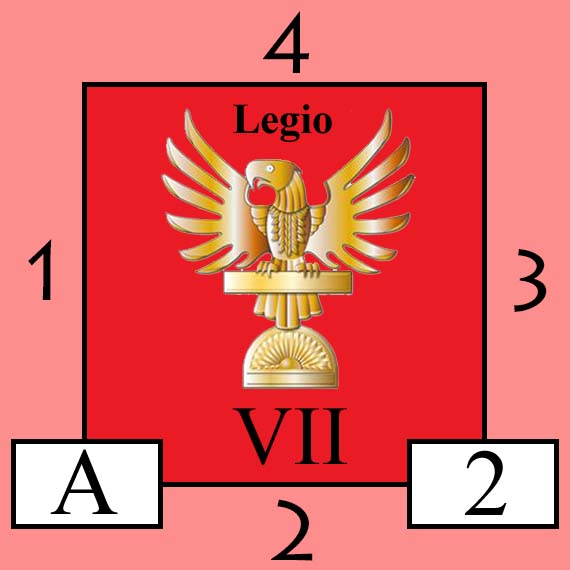
\includegraphics{images/legion7_2nd_ed}
\hspace{1em}
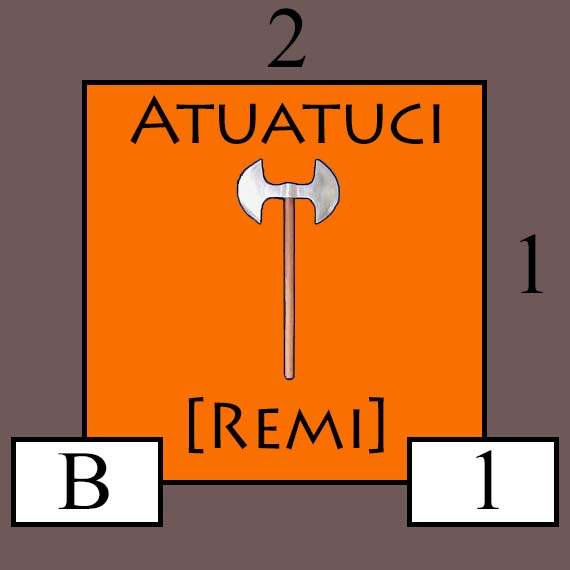
\includegraphics{images/aduatuci_2nd_ed}

\par
\subsection{The Cards}
Cards contain either the name of one or two Barbarian Tribes with an image of their home area on the card, or an event which summarizes the effect of the event. The Action Point value is printed on the card. Note that in one area - Germania - the Action Point value depends on who plays it. It's "2" for the Roman player, but "3" for the Barbarian player.

\section{Game Setup}

The Barbarian player starts with control of the Helvetii tribe at full strength in its home area. Stand this unit up, facing the Barbarian player.

The Roman player starts with six Roman legions in Transalpine Gaul - legions VII, VIII, IX, and X (Caesar) at full strength, as well as legions XI and XII at strength 3 each. The Roman player also controls the Volcae tribe at full strength in its home area, and the Allobroges tribe at strength 1 in its home area. Stand these units up, facing the Roman player.

\textit{Legions XI and XII had been recruited shortly before Caesar began his campaign and so their strength has been reduced to represent their lack of experience. Historically Caesar used them in a reserve capacity the first year. (Book I, Chapter 24)}

The Roman player starts with 15 supply points. Use the provided markers on the general records track supply points throughout the game.

All other Gallic tribes are placed face down in their home areas. They begin the game neutral. As these units become active, they should be stood upright, with the label facing the controlling player.

There are several Gallic areas that list two tribes as their home area. If the names are separated by a slash, such as "Menapi / Nervii" then only one of those tribes will start the game in play. Randomly select one of the tribes for that home area, and set aside the other tribe for now. Both players may know which tribe was selected, and while still neutral it can be inspected if you forget. If the names are separated by a plus sign such as "Bellovaci + Caletes", then both blocks are placed in that area and treat that space as their home area.
\section{Sequence of Play}

The game is divided into 8 turns with each turn representing one year. Each game turn is divided into two phases - a Card Phase, where cards are dealt and played, and an End of Turn phase that is conducted after all cards have been played.

The Card Phase is the main phase of the turn. It consists of drawing cards, playing cards, and resolving actions based on the cards played. The Card Phase is where most of the game's actions take place, including activating neutral tribes, moving units, and performing political actions.

The End of Turn phase is where the game state is updated based on the actions taken during the Card Phase. This includes checking the harvest, replacing units, resolving supply and attrition, and scoring victory points.

The Sequence of Play summary is:

\begin{samepage}
\renewcommand{\labelenumii}{\Alph{enumii}.}
\begin{enumerate}
    \item CARD PHASE
    \begin{enumerate}
        \item Draw Cards and Play
        \item Card Action Phase Order
        \begin{enumerate}
            \item Events
            \item Supply Action
            \item Neutral Tribe Activation
            \item Political Action
            \item Movement
        \end{enumerate}
    \end{enumerate}
    \item END OF TURN PHASE
    \begin{enumerate}
        \item Check Harvest
        \item German and Gallic Replacements
        \item Units Go Home in the following order:
        \begin{enumerate}
            \item Eliminated Gallic Tribe Units
            \item Roman Legions
            \item Gallic Tribes allied to the Roman player
            \item Gallic Tribes allied to the Barbarian player
            \item Germanic units
        \end{enumerate}
        \item Supply and Attrition
        \item Roman Replacements and Reorganization
        \item Roman Supply Point production
        \item Roman Reinforcements
        \item Score Victory Points
    \end{enumerate}
\end{enumerate}
\end{samepage}
\section{Card Phase}
\subsection{Draw Cards}
Shuffle the card deck and deal five cards to each player, shuffling in any cards played from previous turns first.

\textbf{Exception:} Only deal four cards to each player on the first turn of the game.

If the Romans have scored at least 80 victory points, and at least 13 Gallic tribes are Roman allied, the Barbarian player has the option of putting the Massive Revolt card in his hand. If this option is used, only deal four additional cards to the Barbarian player.

If not already played, at the start of 52 BC (only), the Barbarian player may select the Massive Revolt card, even if the Romans do not meet the minimum VP and/or allied Gallic tribes. However, if this option is used, the Roman player receives 1 VP instantly. In addition, it must be the first card played by the Barbarian player, and must be played as an event.

\subsection{Card Action Phase}
Each player selects one card from their hand and places that card face down. Both players then simultaneously reveal which card they have selected. Each player then announces what action they are taking, Romans first. Actions are then resolved in card action order.

There are possible actions and they are resolved in the following order: Event, Supply Action, Neutral Tribe Activation, Political Action, or Movement. If both players select the same action, the Romans resolve their action first.

\textbf{Exception:} If both players selected a Movement action, the player who played a card with the highest action value moves first. If both players played a card with the same action value, the Romans move first.

At the end of each card play, i.e. both players have played their selected card and completed their action, a battle occurs in each area where both players have units they control in the same area. See the "Battle" rules section for more details.

This process is repeated until all cards have been played and resolved. Played cards should be placed into the discard pile unless used for a Neutral Tribe Activation, in which case they should be placed in the player's respective Neutral Tribe Activation area on the map.

Cards cannot be held between turns, i.e. a player may not pass in order to save a card for a future turn. Discard piles are not secret, and may be examined at any time by either player.

All played cards and the unused portion of the deck are shuffled together at the end of the turn for use at the start of the next turn.

\subsubsection{Card Action Phase Order}

\textbf{A. Events}
\par
There are five event cards in the game. Each event card may be played for the event as described on the card, or may instead be played as a 1 for a Movement Action. Event cards may never be used for a Political Action, Neutral Tribe Activation, or Supply Action. The cards explain the event and how it is applied to the game for each player. See the card roster section at the back of the rules for a more detailed explanation of each event.

\textbf{B. Supply Action}
\par
The Roman player tracks supply points on the General Records track on the game board using the Roman Supply block. The Roman player may add a number of supply points equal to double the Action Point value of the card.

\textit{Example: The Roman player uses the Germania card (3 action points) for a supply action. The Roman player adds 6 supply points (3 x 2) to the supply track.}

The Barbarian player may not use a card for a Supply Action until the leader Vercingetorix is in play. The Barbarian player's version of a supply action is to \textbf{reduce} the number of Roman supply points by the Action Point value of the card. Unlike the Roman player, this value is NOT doubled.

The Barbarian player may perform a maximum of one Supply Action per year, whereas the Roman player can perform as many Supply Actions as desired.

\textbf{C. Neutral Tribe Activation}
\par
Both players may activate neutral tribes and automatically bring them under their control as allies at full strength. The name of the home area on the card must match the name of neutral tribe's home area that the active player wishes to activate. When neutral tribes are activated, stand the unit(s) upright, facing the player to which they are now allied. In areas that have two tribes, both tribes are activated.

Neither player can change control of a tribe that is already controlled by the opposing player with a Neutral Tribe Activation. The Barbarian player is limited to two Neutral Tribe Activations per year, while the Roman player is limited to one Neutral Tribe Activation per year.

\textbf{Exception:} The Roman player may not use a Neutral Tribe Activation to activate any units in Britannia or Germania.

\textbf{D. Political Action}
\par
Either player may use a card to attempt to change the political allegiance of any Gallic tribe on the board, whether it's neutral or controlled by the opposing player.

Roll a die. If the selected area of the Political Action matches the home area on the card, the active player receives a -1 bonus to the die roll. If the inactive player controls a unit that is in that area, then the active player receives a +1 penalty to the die roll.

If the die roll is less than or equal to the Action Point value on the card played, the Political Action is successful and control of that area is switched to the active player. The Gallic tribe's block is immediately returned to its home area (if not already home) at its current strength. This is not considered movement, simply pick up the block and put it in their home area.

If there are enemy units present then a battle is immediately fought (see 5.2.2 Battles). The units returning home are considered the attacker, and follow the standard rules for battle, i.e. 3 rounds of combat, and must retreat if there are still defending units at the end of 3 rounds, etc.

If the area is home to multiple units, then a successful political action is considered successful against all units of that area. They all return home as a single force.

If a Political Action is successful against the home area of a Minor Leader, that leader is immediately removed. If a Political Action is successful  against the home area of Vercingetorix, the Barbarian player immediately designates a new home area for him. The newly selected area must belong to a tribe that is currently controlled by the Barbarian player and is free of enemy units. If no such area exists, then Vercingetorix is eliminated. The Roman player scores VP normally in this case.

\textbf{Exceptions:} Neither the Roman player nor the Barbarian player may target Britannia as the target of a Political Action unless there is at least one Roman legion (Romans), or a leader (Barbarians), in a port area connected to Oceanus Britannicus. The Roman player may not use a Political Action against Germania.

A neutral tribe activated by a Political Action does not count against the Neutral Tribe Activation limit.

\textbf{E. Movement}
\par
The active player may activate for movement a number of groups up to the Action Point value of a card, or none at all if they choose. All units within an area area considered a group. Each group moving may move together to the same area or individual units within the group could move to separate areas. Unit movement rate is one area per card play. Retreat and regroup do not count as movement. All groups must be designated prior to actual movement.

\textit{For example, 4 Roman legions starting in Transalpine Gaul could as part of one group move have 2 units move into Allobroges and 2 units move into Helvetii, or all 4 into Allobroges, or any number of other moves within the restrictions of movement.}

\textbf{Exception:} Each Roman legion unit in the off-map area is considered its own group, i.e. they must be moved onto the map one at a time, and only into Transalpine Gaul. Barbarian units may not enter the off-map area.
\par
Borders and other terrain restrict movement and limit the number of units that may move from one area to another adjacent one. A maximum of four units may cross a black border from one area to another. A maximum of two units may cross a blue border from one area to another. Border limits are applied separately to each player. For example, both the Roman and Barbarian player could move two units across the same blue border in the same card play.

All units crossing a blue border, moving using naval movement, or which enter an area containing enemy or neutral units must stop immediately. This supersedes forced marches by Roman units, i.e. a supply point may not be spent to force march a Roman unit that has just crossed a blue border (though it could cross a blue border on its second move).

Units moving into an area containing enemy or neutral units are considered to be the attacker. Units already in an area which the opposing player moves units into are considered the defender. Entering an area that contains a neutral tribe on the board causes that tribe to join the opposing player, though battle is not resolved until the end of the card play round. If both players move into the area of a neutral tribe, the tribe will join the player who moved into the area last.

\textit{\textbf{Pinning:}} When moving into an area, all attacking units (including reserves, see below) prevent an equal number of defending enemy units from moving in that round. The defender chooses which units are pinned. Any unpinned units may move and attack normally, except that they may not cross any border used by the attacker to enter that area.

\textit{\textbf{Roman Unit Force March:}} Roman legion units have the option to expend one supply per unit in order to conduct a forced march. This allows the Roman legion to move up to two areas per card play instead of one.

\textbf{CROSSING THE RHINE}
\par
Only German units and Roman legion units may cross the Rhine. Gallic tribes may not cross the Rhine.

\textbf{Exception:} Roman units may not cross the Rhine into Germania if there are no German units there.

\textbf{NAVAL MOVEMENT}
\par
An ocean area may not be entered or crossed except from port area to port area using naval movement. Only units that start in a port area may use naval movement. Up to two units may move from one port area to another port area within the same sea zone as part of one group move.

Note: Units that start in the Osismi area may move across either sea zone since it is considered to have a port in both sea zones.

Barbarian units may not use naval movement to enter a port that contains enemy or neutral units. Conversely, Roman units may use naval movement to enter a port area that contains neutral or enemy units at the cost of 1 supply point per group.

See the Battle rules for special rules during an amphibious invasion 

\textbf{STACKING AND ATTRITION}
\par
There is no limit to the number of blocks that may occupy an area on the map. However, if a player has more than 6 blocks in an area at the end of their card play (i.e. after all movement, combat and regrouping has occurred), then each block in excess of 6 takes one point of attrition damage.

\textbf{Exception:} Roman legions do not count against the stacking limit in Transalpine Gaul. There is no stacking limit in the Roman off-map area.

The owning player may choose which units take step losses, but may not eliminate a block if possible, and Gallic non-leader units must take losses prior to Roman, German or Gallic leader units.

\textbf{Movement Example}
\par
\textit{The Roman player used a '1' action point card for movement, and may thus activate one group (area). He activates the group in Transalpine Gaul since his six legions are all there. He moves legion VII and VIII directly from Transalpine Gaul into the Helvetii area. Since it's a blue border he cannot move any more units across that border. He then uses two supply points to force march legions IX and X (Caesar) from Transalpine Gaul to Allobroges, and from there into Helvetii. Roman supply is reduced from 15 to 13.}
\par
\textit{The Romans then force march legions XI and XII from Transalpine Gaul to Sequani through Allobroges. Roman supply is reduced from 13 to 11. The Roman legions can force march through Allobroges because the Gallic units in Allobroges are Roman allies. If the Roman player had played a '2' action point card, he could also have moved the Roman allies in Allobroges or any other group in an area.}

\section{Battle}
\par
Battles are fought as a result of Event, Political Action and Movement card play. Each battle must be completed before fighting the next battle. Battles occurring as the result of Event and Political Action card play are resolved immediately with the order determined by the active player. The player who selected a movement action and moved first this round determines the order in which battles are fought as the result of a movement card play.

In any area in which there is a battle both players reveal their units by tipping their blocks forward so that they show their current strength. After each battle is completed, return any surviving units upright before proceeding to the next battle. After all units have taken one battle action, one battle round is considered to have passed. Repeat the sequence for a 2nd and 3rd round if necessary.

Most battles are fought for a maximum of 3 battle rounds, though when crossing the Rhine into Germania or amphibiously invading an area there are only 2 battle rounds. The attacker must retreat if the defender is not eliminated and does not retreat at the end of the maximum number of battle rounds. This procedure is repeated until all battles are complete.

Each unit may fire, retreat or pass during each battle round. This is called a battle action. The order in which a unit resolves its battle action depends on its initiative. Any defending units with an "B" initiative take their battle action first, followed by all attacking "B" units. Then all defending "C" units take their action, followed by all attacking "C" units. Finally, all defending "D" units take their action, followed by all attacking "D" units.

\textbf{Note:} If the Caesar unit (Legion X) is involved in a battle, it always takes its action first, regardless of enemy initiative or circumstances, since it is the only "A" rated block.

Each unit may “fire” by rolling as many dice as its strength. A hit is scored for every roll less than or equal to its battle rating. Against most units each hit reduces an enemy unit by one strength point. This is indicated by rotating the unit counter-clockwise for each hit. Enemy units may not be targeted individually. Each hit is applied to the strongest enemy unit. If two or more enemy units are the same strength, the owner decides on which unit to apply the hit. Units eliminated in battle are set aside until the End of Turn Phase.

\textbf{Exceptions:} In mixed forces, Roman or German units must take a hit before allied Barbarian units if they have the same strength.

Some units require two hits to be reduced by one strength. If possible, all hits must be applied. If an odd number of hits remain at the end of a battle round after applying all hits, the excess are ignored, except in sieges. See below.

\textbf{A. Reserves}

Multiple groups may attack or defend the same area, moving across the same or different borders. However, only one group is considered the main group. All other groups are considered reserves. In the case of defending units, the units that began the action in an area are considered the main group. Any units that moved to help defend the area are considered reserves. In the case of attacking units, the players attacking an area decides which group is the main group and which groups are reserves.

Reserve units may not perform a battle action or suffer hits, nor are they revealed, in the first round of battle. They are revealed and participate in the 2nd round of battle, even if all other friendly units have been eliminated. If the attacking player eliminates all defending units before defending reserve units arrive, then the original attacker is now considered the defender, and the original defender is now considered the attacker. Battle is then resolved normally.

\textbf{B. Sieges}
\par
Defending units that start a battle in an area with a fortress may declare that they are inside the fortress, up to the limit of the supply value of the fortress. Thus, most fortresses may only hold one unit, while Transalpine Gaul and Avaricum can hold up to two units. Defending reserve units do not have this option.

If a Gallic unit is defending in its home area with a fortress, then that unit must be chosen first over other potential units to defend inside a fortress, if any are chosen at all. If there is more than one Gallic unit defending its home area, then the owning player may choose which one goes inside the fortress, and the other unit must fight outside the fortress.

In the circumstance where there are defending units both outside and inside a fortress, a battle is fought normally against the outside unit(s) first. If the attackers successfully defeat the outside units within 3 battle rounds, either by eliminating them or forcing them to retreat, then the attacker has the option of either assaulting the fortress or retreating. If retreat is chosen at this point, it happens prior to the defender rolling any dice.

If the attacker chooses to assault, then the attacker gets a fresh set of 3 battle rounds to prosecute the assault. If the assault is not successfully completed within the allotted number of rounds, then the attacker must retreat.

Units defending in a fortress against an assault are treated as having an "B" initiative. In addition, the defending unit has double defense, i.e. it requires two hits to score one point of damage. Leftover hits are retained between battle rounds, but are discarded once the assault is over.

Defending units inside a fortress may not retreat or reorganize after battle unless the attacking units retreated or were eliminated first.


\textit{Designer's Note: Note that I deliberately do not use a "siege point" system that is popular with other ancients games. Historically the Roman sieges of the various Gallic fortified towns were very brief, and were usually resolved by the Romans cutting off their enemy's food and water supply. Once that was accomplished, the barbarians would soon surrender.}

\textit{The largest and longest sieges of the campaign at Avaricum and Alesia lasted just a few weeks, but most seem to have been successfully prosecuted within a few days. For this reason I do not provide siege rules that are more detailed because they simply wouldn't be appropriate at this scale.}

\textbf{B2. Reserve Units Entering a Besieged Area}

If reserve units are entering an area that would normally be under siege, instead the Reserve units arrive instantly. Skip round 1 of combat and proceed directly to round 2, and fight a field battle, with sieging units considered the defender. 

Any besieged units may optionally sortie out to join their Reserve forces in this situation, but if they elect to retreat then they may only retreat back into the fortress.

Once resolved, the sieging units may proceed with the siege normally, assuming they win the battle.

\textit{Example: On the Roman player's turn, four Roman legions have entered the Mandubii home area. Vercingetorix is the only unit there, with the Mandubii and Senones units having retreated to an adjacent area earlier in the turn. Vercingetorix retreats into the fortress (Alesia).}

\textit{Normally a siege would result. However, the Barbarian player has moved four Gallic units into the area from adjacent areas on his turn to try and save Vercingetorix, making them Reserve units entering a besieged area. Consequently, the Roman legions are now defending units against attacking Barbarian units as if it were the start of round 2 of battle. The Barbarian player elects to sortie out Vercingetorix to join the fight.}

\textit{Unfortunately for the Barbarian player, the attack does not go well, and after two rounds of combat (rounds 2 and 3) they are unable to force the Romans to retreat. Since a 3rd round of battle has been fought, the Barbarian units that entered as Reserves are forced to retreat. Vercingetorix retreats back into the fortress since he sortied out.}

\textit{With the field battle now complete, the Romans may conduct a siege normally, i.e. they get a fresh set of rounds to conduct the siege.}

\textbf{C. Crossing the Rhine Into Battle}
\par
When the Romans or Germans cross the Rhine into Germania or a Gallic area the ensuing battle is restricted to a maximum of two rounds instead of the normal three.

This restriction only applies if the main group attacked across the Rhine. It does not apply if only reserves crossed the Rhine.

Every German unit killed in battle immediately scores 1 VP for the Roman player, except Ariovistus, which scores 2 VP for the Roman player.

\textbf{Germanic Strategic Withdrawal Option}
\par
The Barbarian player may strategically withdraw any or all German units in Germania, including Ariovistus, from the board before battle begins. This is not like a retreat, the units are not moved to a friendly area. Instead they are removed from the game.

Every German unit that strategically withdraws does not score any VP for the Roman player, but it is then permanently removed from the game.

Note that the strategic withdrawal option is only available for German units in Germania. It does not apply to German units fighting outside of Germania, and it can only be taken prior to battle. Once battle begins, the option to strategically withdraw is no longer available.

\textit{Designer's Note: This is designed to simulate the strategic value of Caesar's raids across the Rhine. Historically, these did not cause much in the way of actual damage or casualties because the Germanic tribes withdrew rather than risk a pitched battle. What it did accomplish, however, was to demonstrate to the Germans that the Romans could cross the Rhine at any time, and effectively convince them not to cross the Rhine into Gaul again.}
\par
\textit{Thus, the Barbarian player has to make a choice whether to risk giving the Roman player more VP's through a pitched battle, or to minimize the Roman VP potential at the cost of permanently losing control of German units.}

\textbf{D. The Alps}
\par
Units defending in the Alps (the Helvetii/Nantuates home area) receive double defense, i.e. it requires two hits in battle to score one point of damage.

\textbf{E. Amphibious Invasions}
\par
Barbarian units defending against Roman units that entered the area via naval movement are all treated as having a "B" initiative rating. In addition, there are only two rounds of battle instead of the normal three (and two rounds of siege instead of the normal three if a fort is present). 

This only applies if the main force entered by naval movement. If a reserve force entered by sea, but the main force entered by land, then fight the battle normally. 

\textbf{F. Retreat}
\par
Instead of firing, each unit may retreat to an adjacent friendly or empty area, or into a fortress if the area contains one and there is room for it. Units may retreat to the same or different areas. Retreating units are returned to their face up position before retreating, potentially concealing which units are retreating to any particular area. Border limits apply to retreating units on a per-battle-round basis, e.g. four units could retreat across a blue border, but no more than 2 per battle round

Units may not retreat into an area through which enemy units entered the area. However, if both players moved units across the same border in the same round, only the player who crossed the border last may retreat across that border.

Units may not retreat into a contested area, i.e. an area where there is an unfought battle. Only German units may retreat into Germania.

\textbf{Naval Retreat}
\par
Roman units conducting a naval move into an enemy port may retreat to any friendly port area in the same sea zone. They may not retreat if there is no friendly port area in the same sea zone.

Any units defending in a port area may retreat up to two units (maximum, not per battle round) to another friendly port area in the same sea zone.

\textbf{G. Regroup}
\par
The player left controlling the area at the end of battle is considered the victor and may regroup surviving units. Regroup allows all victorious units, including any in reserve, to move to any adjacent friendly or empty area.

A Unit cannot regroup into an unfought battle. Only German units may regroup into Germania. Border limits apply to regrouping units.

Roman units (only) in a port area may regroup into a friendly or empty port area in the same sea zone, up to a maximum of two units per area.
\section{End of Turn}
\par
After all cards have been played (i.e. the Card Phase is completed for the the year), players must now deal with returning units to their home areas, supply and replacements. This reflects the end of the campaign year when armies returned home or went into winter quarters in effect “wintering”. The End of Turn sequence below should be followed strictly.

\subsection{Check Harvest}
\blockquote[Book V, Chapter 24]{The grain harvest that year in Gaul had been poor because of drought, so I was compelled to change my usual methods of arranging winter quarters for my legions, and distribute them among a larger number of tribes.}
\par
The harvest affects garrison limits for each area at the end of the year. Check the harvest by rolling a die.

On a roll of 1, it’s a poor harvest and the garrison limit for each area is 1 legion. Immediately reduce Roman supply by 2 points.

On a roll of 6, it’s a bountiful harvest and the garrison limit for each area is 3 legions. Immediately increase Roman supply by 2 points.

On a roll of 2-5 the garrison limit for each area is 2, and there is no adjustment to the Roman supply track.

Caesar and Gallic tribe units (including minor leaders) in their home area do not count against the area garrison limit.

\raggedbottom

\subsection{German and Gallic Replacements}
\par
German units in Germania and Gallic tribe units controlled by either player in their home area may add one point strength per unit. Gallic and German units outside of their home area may not receive replacements.

\textit{Note: Since eliminated German and Gallic units are not on the board yet, they do not have the opportunity to receive replacements this turn.}

\begin{samepage}
\subsection{Units Go Home}
\par
Units return to their home areas in the following order:
\begin{enumerate}
  \setlength\itemsep{0em}
  \item {\small Eliminated Gallic units}
  \item {\small Roman legions}
  \item {\small Gallic units controlled by the Roman player}
  \item {\small Gallic units controlled by the Barbarian player}
  \item {\small German units}
\end{enumerate}
\end{samepage}

\subsubsection{Eliminated Gallic Units Return Home}
\label{eliminated_gallic_units_return_home}
\par
Gallic tribe units that were eliminated return to their home area. If the area is occupied by any units, the tribe is now controlled by the owner of the occupying units at strength 1. If the area is not occupied by any units, it returns to neutral status at full strength and the units are placed face down.

\textbf{Exception:} If the Helvetii are eliminated, they are permanently removed from the game. Replace them with the Nantuates unit which returns at full strength (during the "Eliminated Gallic Units Return Home" step), and under the control of any player that occupies the Helvetii area, or face down if neither player does.

\subsubsection{Roman Legions Return Home}
\blockquote[Book V, Chapter 53]{Caesar sent Fabius back to his winter quarters with his own legion, while he himself decided to spend the winter with three legions, each in its own camp, around Samarobriva. Since such formidable Gallic uprisings had occurred, he thought it best to remain personally near the army for the entire winter.}
\par
All Roman legions returning home must return to Transalpine Gaul. If there are enemy units in Transalpine Gaul, then a battle is resolved immediately. All returning legions are considered a single group, and are considered the attackers. Barbarian units eliminated in battle return home as per \ref{eliminated_gallic_units_return_home} and \ref{german_units_return_home}, respectively, at the end of the battle. Roman units may only retreat or regroup to the Off-Map area, if necessary.

Caesar must return home if he stayed outside of Transalpine Gaul at the end of the previous turn. Use the ‘Caesar Wintered’ block on the turn track to remind yourself if and when the Caesar unit remains outside Transalpine Gaul at the end of a year. If Caesar must return to Transalpine Gaul but is stopped because he is unable (or unwilling) to defeat Barbarian units already there, then upon retreat he returns to the off-map area instead.

The Roman player may leave a number of legions in Gallic areas outside of Transalpine Gaul up to the garrison limit of each area. Each legion that does not go home costs Supply points as per \ref{supply_and_attrition}. Each legion suffers a 1 step reduction on its strength if a Supply point cannot be paid, except for the Caesar unit which may stay in any Gallic tribe area at no Supply cost and does not count against an area's garrison limit. Roman legions that have been eliminated do not return immediately, but instead return as reinforcements the following turn. See the Roman Reinforcements section eliminated Roman legions.

Any legions currently in the Off-Map area may move for free into to the Transalpine Gaul area, potentially participating in a battle there as a reserve force.

Legions may not winter in Germania.

\subsubsection{Gallic Units Controlled by the Roman Player Return Home}
\par
Gallic tribe units controlled by the Roman player return home and remain Roman allies. If their home area is occupied by units controlled by the Barbarian player, they switch allegiance to the Barbarian player immediately at current strength.

\subsubsection{Gallic Units Controlled by the Barbarian Player Return Home}
\par
Gallic tribe units, including minor leaders, controlled by the Barbarian player then return to their home area (unless staying outside of their home area with Vercingetorix) and remain Barbarian allies. If the area is occupied by a Roman unit or Roman allied Gallic unit then the tribe defects at current strength to the Roman player. If the home area of a minor leader is occupied by a Roman legion, then the minor leader is eliminated instead. Vercingetorix may return to his home area but is not obligated to, since he can stay outside of his home area every turn. Gallic tribe units may only remain outside of their home area if they remain with Vercingetorix, up to the garrison limit of the area.

\textit{Note: Unlike Caesar, Vercingetorix counts against the area's garrison limit.}

\textbf{Exception:} If the Helvetii unit was eliminated, replace it with the Nantuates unit at full strength instead.

\subsubsection{German Units Return Home}
\label{german_units_return_home}
\par
German units that were eliminated return to Germania at strength 1. German units (only) may remain with the Ariovistus unit outside of Germania up to the garrison limit of the area. All other German units return home at their current strength.

The Ariovistus unit does count against the area garrison limit. Use the ‘Ariovistus Wintered’ block on the turn track if Ariovistus remains outside of Germania at the end of a year. Ariovistus must return home if he stayed outside of Germania at the end of the previous turn.

\textbf{Note:} Roman and Gallic units, including leaders, may not stay in Germania at the end of a turn.

\subsection{Supply and Attrition}
\label{supply_and_attrition}
\par
The Roman player must now pay Supply points for each Roman legion wintering outside of Transalpine Gaul. It always costs 1 Supply point per legion, regardless of the Harvest level. If enough supply points are not available, each legion that cannot be supplied takes one step reduction through attrition.

The Roman player must attempt to supply all units. Attrition is never voluntary. Any legions reduced to strength 0 from attrition are eliminated and count as victory points for the Barbarian player. Any legion eliminated as the result of attrition will return at the end of the following turn as a reinforcement. See the Roman Reinforcements section at \ref{roman_reinforcements} for more details.

\textit{Note: If this is the last turn, you can skip ahead to Score Victory Points from here.}

\subsection{Roman Replacements}
\par
The Roman player may add strength steps to Roman legions using supply points. Each step added costs one supply point. Legions outside of Transalpine Gaul may only add a maximum of one step per unit. Legions in Transalpine Gaul or the Off-Map area may add strength steps up to their maximum strength.

\subsection{Roman Supply Point Production}
\par
The Roman player now receives one Supply point for each fortified town area he controls, except for Transalpine Gaul and Avaricum, which each produce two Supply points. Adjust the Roman Supply block accordingly. The number of Supply points may never increase above 19, nor decrease below 0.

\subsection{Roman Reinforcements}\label{roman_reinforcements}
\blockquote[Book II, Chapter 2]{This news as well as dispatches prompted Caesar to levy two new legions in Cisalpine Gaul, and by the beginning of the milder season he sent his legate Quintus Pedius to lead them into the interior of Gaul.}
\par
After collecting supply points, the Roman player has up to three new legions that can be constructed. The cost is one supply point per strength point, up to four strength points, maximum (though less if desired). These are legions XIII, XIV, and XV. Normally a maximum of one new legion per turn may be brought in as a reinforcement.

If the Massive Revolt event has been played then two additional units - legions V and VI - may be built by the Roman player, and for the rest of the game up to two legions per turn can be brought in as reinforcements.

Any reinforcements, including eliminated legions returning to play, are placed in the Roman Off-Map area.

\subsubsection{Eliminated Legions}
\par
Any Roman Legions that were eliminated this turn return at the end of the next turn during the Reinforcement Phase at full strength in the Roman Off-Map area. For example, a legion killed on turn 3 (56 BC) would return at the end of turn 4 (55 BC). Players should place eliminated legions on the turn track to indicate when they will return to play.

Legions that are eliminated and return to play in this manner do not require supply points to replace.

\textit{It is assumed that if the legion is destroyed that Caesar received a replacement legion from Rome. This happened historically when 15 cohorts were destroyed in 54 BC, and a legion - borrowed from Pompey - was sent to replace it.}

\subsection{Score Victory Points}
\par
The Roman player now scores victory points for controlled tribes. These points are cumulative with points scored on previous turns.

Each controlled tribal area scores 1 VP for the Roman player. Remember that this does NOT include Transalpine Gaul.

\textit{For VP purposes, this does not include Transalpine Gaul or the Roman off-map area.}

\subsection{Score Optional VP}
If playing with the Yearly Objectives optional rules, score those points as appropriate now. See the section on Yearly Objectives for more details.

\section{Leaders}
\par
A few units represent significant historical figures at this time. They are integrated into units, rather than having separate units. Some leaders have special abilities.

\subsection{Julius Caesar}
\par
Legion X (the tenth legion) represents Julius Caesar. Caesar’s unit always activates first regardless of the initiative rating of defending units or other special rules.

In addition, Caesar’s unit does not count against an area’s garrison limit.

If Legion X is eliminated (i.e. Julius Caesar is killed) then the Barbarian player instantly wins an automatic victory.

\subsection{Ariovistus}
\blockquote[Book I, Chapter 31]{Things had turned out worse for the victorious Sequani than for the vanquished Aedui. Ariovistus, the king of the Germans, had settled in their territory and had seized a third of their land, the best in the whole of Gaul.}
\par
Ariovistus was a king of the Germans. His name is written on his unit to distinguish him from other German units. He begins the game in Germania, which is his home area.

When Ariovistus attacks a neutral area, first roll a die for each neutral Gallic unit. On a 1-2, that tribe joins the Barbarian player automatically and no battle is fought against that unit. The Barbarian player may then regroup normally. If the Ariovistus unit is eliminated (i.e. Ariovistus is killed), then he is removed from the game permanently.

Note that it is possible that, in an area with multiple tribes, one Gallic unit could join the Barbarian player while the other does not. In that case, the tribe that joined the Barbarian player would be considered part of the main attacking force against the remaining unit.

\subsection{Vercingetorix}
\par
Vercingetorix appears as a result of the play of the Massive Revolt event card by the Barbarian player and he is always allied to the Barbarian player.

The Barbarian player receives a -1 die roll bonus modifier on all Political Action attempts if the attempt is made against a tribe whose home area is adjacent to the Vercingetorix unit. If this ability is used then the Barbarian player must announce the location (but not strength) of Vercingetorix. This ability is optional. The Barbarian player may forfeit the bonus and resolve a Political Action normally in order to avoid revealing the location of Vercingetorix.

Vercingetorix may remain outside of his home area every turn. He is not obligated to return to his home area. Any Gallic tribe (but not German) units in the same area as Vercingetorix at the end of the turn may remain in the same area as Vercingetorix, so long as they don’t exceed the area’s garrison limit.

\textbf{Note:} This is the only time Gallic tribe units may remain outside of their home area at the end of the turn.

While Vercingetorix is in play the Barbarian player may conduct one Supply Action (raid) per turn. If Vercingetorix is eliminated, he is removed from the game permanently.

\subsection{Minor Gallic Leaders}
\par
There are two minor Gallic leader units, Dumnorix and Ambiorix, which can appear as the result of the play of the Major Revolt event card by the Barbarian player. They are always allied to the Barbarian player. Minor leaders have no special abilities. They are merely an extra unit for the Barbarian player.

Minor Gallic leaders may never be controlled by the Roman player. Although the minor leaders have been given names for historical flavor, they are not permanently eliminated from the game if removed during play. A minor leader could be eliminated and later return through the play of another Major Revolt card. There are two home area markers for the minor leaders to place and keep track of where their home areas are.

\textit{These leaders abstractly represent various Gallic leaders that would crop up from time to time and stir up trouble against the Romans.}

\section{Victory Conditions}
\par
The Barbarian player wins instantly if Caesar is killed. Otherwise, victory is checked at the end of turn 8 (51 BC).

If the Roman player has scored at least 90 victory points, then the Roman player has scored a Minor Victory. Caesar returns to Rome, receives an Ovation and manages to avoid prosecution thanks to a modicum of popularity. However, his career wanes after that, and he fades into obscurity.

If the Roman player has scored at least 100 victory points, then the Roman player has scored a Major Victory. Caesar returns to Rome, receives a Triumph, 
and easily defeats prosecution attempts. Within a few years he leads an invasion against the Parthian Empire.

If the Roman player has scored at least 110 victory points, then the Roman player as scored a Massive Victory. History repeats itself. Caesar takes an army into Italy and the die is cast.

If the Roman player has scored less than 90 victory points then Barbarian player is considered victorious. Caesar returns to Rome without an army and is successfully prosecuted for crimes during his consulship. His senatorial career is over.

In addition to the cumulative end of turn VP scored, the following events also affect the Roman player's VP score:

\begin{itemize}
  \setlength\itemsep{0em}
  \item Each German non-leader unit eliminated: +1 VP
  \item Ariovistus eliminated: +2 VP
  \item Vercingetorix eliminated: +3 VP
  \item Amphibiously invade Britannia with at least 2 legions and fight at least one round of combat: +2 VP*
  \item Invade Germania with at least 2 legions and fight at least one round of combat and/or force at least one German unit to withdraw: +2 VP*
  \item Each Gallic home unit in Britannia eliminated: +1 VP (max 2 VP)*
  \item Each Roman legion unit eliminated: -5 VP
\end{itemize}

Note that the points for invading Britannia and Germania can only be scored once during the game. The number of VP for killing Gallic home units in Britannia is restricted to a maximum of 2 VP.

* Ignore this if playing with the optional Yearly Objectives.
\section{Yearly Objectives}
This is an optional rule designed to steer players towards the actual historical results. The sections below are broken down per year, with a title briefly describing the major events and/or historical figures of that year.

At the end of each turn at the end of the Score Victory Points phase, after scoring points normally, the Roman player may gain or lose additional victory points as the result of certain conditions. Those conditions are dependent on the turn, and are described below. It is possible that more than one condition applies, in which case the Roman player should gain bonus VP first, then apply lost VP afterwards.

\subsection{Turn 1 (58 BC): Ariovistus}
\begin{itemize}
  \setlength\itemsep{0em}
  \item The Roman player controls Sequani, Allobroges and Helvetii/Nantuates territory at the end of the turn: +1 VP
  \item The Barbarian player controls Sequani territory at the end of the turn: -1 VP
  \item The Helvetii unit has not been destroyed by the end of the turn: -1 VP
\end{itemize}

\subsection{Turn 2 (57 BC): The Belgic Campaign}
\begin{itemize}
  \setlength\itemsep{0em}
  \item The Roman player controls at least 3 territories adjacent to Oceanus Britannicus: +1 VP
  \item The Roman player controls the Remi/Aduatuci territory: +1 VP
  \item The Barbarian player controls at least 3 territories adjacent to Oceanus Britannicus: -1 VP
\end{itemize}

\subsection{Turn 3 (56 BC): Galba, Crassus and the Venetic Campaign}
\begin{itemize}
  \setlength\itemsep{0em}
  \item The Roman player controls the Helvetii/Nantuates territory and garrisons at least one legion there at the end of the turn: +1 VP
  \item The Roman player controls both the Osismi and Veneti territories: +1 VP
  \item The Roman player controls at least one tribe in Aquitania: +1 VP
  \item The Barbarian player controls the Helvetii/Nantuates territory at the end of the turn: -1 VP
  \item The Barbarian player controls at least one tribe in Aquitania: -1 VP
  \item The Barbarian player controls either the Osismi or Veneti territories: -1 VP each.
\end{itemize}

\subsection{Turn 4 (55 BC): The German Campaign and First Expedition to Britannia}
\begin{itemize}
  \setlength\itemsep{0em}
  \item The Barbarian player controls the Menapi/Nervii territory, or the Atrebates/Morini territory, and winters at least one German unit there at the end of the turn: -2 VP
  \item The Roman player crosses into Germania with at least one Roman legion and fights at least one round of combat: +1 VP
  \item The Roman player crosses into Britannia with at least one Roman legion and fights at least one round of combat: +1 VP
  \item The Roman player controls Britannia at the end of the turn: +1 VP
\end{itemize}

\subsection{Turn 5 (54 BC): Dumnorix, The British Campaign, and Winter Quarters}
\begin{itemize}
  \setlength\itemsep{0em}
  \item The Roman player crosses into Britannia with at least two Roman legions and fights at least one round of combat: +1 VP
  \item The Roman player kills Dumnorix: +1 VP
  \item The Roman player winters with at least one legion in at least four different territories at the end of the turn: +1 VP
  \item The Barbarian player controls Britannia at the end of the turn: -1 VP
  \item The Barbarian player has Dumnorix in play at the end of the turn: -1 VP*
  
*In a 2-player game the Barbarian player must bring Dumnorix into play as the first card played this turn in order for this to apply.
\end{itemize}

\subsection{Turn 6 (53 BC): The Treveri Campaign, Ambiorix, and a raid into Germania}
\begin{itemize}
  \setlength\itemsep{0em}
  \item The Roman player controls the Treveri/Eburones, Remi/Aduatuci, and Menapi/Nervii territories at the end of the turn: +1 VP per area
  \item The Roman player kills Ambiorix: +1 VP
  \item The Roman player crosses into Germania with at least one legion: +1 VP
  \item The Barbarian player controls the Treveri/Eburones, Remi/Aduatuci and Menapi/Nervii territories at the end of the turn: -1 VP per area
  \item The Barbarian player has Ambiorix in play at the end of the turn: -1 VP*
  
*In a 2-player game the Barbarian player must bring Ambiorix into play as the first card played this turn in order for this to apply.
\end{itemize}

\subsection{Turn 7 (52 BC): Vercingetorix}
\begin{itemize}
  \setlength\itemsep{0em}
  \item The Roman player kills Vercingetorix: +2 VP
  \item The Barbarian player controls Vercingetorix and at least four Gallic tribes at the end of the turn: -2 VP*
  \item The Barbarian player has not brought Vercingetorix into play by the end of the turn: +1 VP
  
The Barbarian player must bring Vercingetorix into play as the first card played this turn in order for this to apply.
\end{itemize}

\subsection{Turn 8 (51 BC): Mopping Up}
\begin{itemize}
  \setlength\itemsep{0em}
  \item The Roman player has eliminated or controls at least one tribe in each of Belgica, Aquitania and Celtae: +2 VP
  \item The Barbarian player controls more tribes than the Roman player: -2 VP
\end{itemize}

\section{Optional Rules}
\par

\textbf{Historical Reinforcements}

Instead of constructing legions as desired, the Roman player receives reinforcements on a more or less historical schedule.

The Romans have up to six legions that will enter the game as reinforcements during the course of the game. The legions that can enter are marked on the turn track. The exact turn they enter depends on the turn and, in most cases, a die roll.

Beginning on turn 1 (58 BC) the XIII and XIV legions are eligible to enter the game. On turn 1 they enter on a roll of 1-2. Roll a die for each legion individually. On turn 2 they enter on a roll of 1-3. On turn 4 they both enter automatically if they have not already entered.

Beginning on turn 5 (54 BC) both the I and XV legions are eligible to enter the game. Roll a die for each unit individually. On turn 5 they enter on a roll of 1-3. On turn 6 they enter on a 1-4. On turn 7 they enter automatically if they have not already entered.

Legions V and VI enter the game at the end of any turn in which the Massive Revolt event is played, and Vercingetorix was brought into play.

\textit{Historically Caesar finished the campaign with 11 legions. He originally started with four legions - VII, VIII, IX and X - but recruited two more legions before launching his campaign, legions XI and XII (Book 1, Chapter 24). The following winter he recruited two more legions - XIII and XIV (Book 2, Chapter 2). Pompey loaned Legion I to Caesar after legion XIV was destroyed. Legions V and VI were recruited in response to Vercingetorix in 52 BC.}
\section{Solitaire Rules}

If you wish to play this game solitaire, then you will play as the Romans and attempt to match Caesar's historical accomplishments. Some changes to setup apply, as well as special rules that will govern how the Barbarian "bot" behaves.

Since you are playing solitaire, you may play with your units face up if you wish. However, to avoid potentially confusing your own units with other units, all enemy units should remain hidden and pointed away from you until the area is activated for movement and potential attacks.

In most cases you will roll on the Random Tribe Selection table when asked to randomly select an area. However, in other cases the instructions will simply state that you should "randomly determine" one or more areas. If this is the case then you must devise a reasonable way to randomly select from multiple areas or units.

\textit{For example, for the Massive Revolt event, the second tribe selected must be an adjacent area which is randomly determined based on the results of the first roll. If there were three adjacent areas that were all viable options, then you could assign 1-2 to one, 3-4 to another, and 5-6 to another. Then roll 1d6 to determine which one is actually selected.}

SETUP

Deal cards only to yourself, the Roman player, at the start of each turn as per the two player rules. In the solitaire version cards are not played simultaneously, but one at a time. You will play a card and then, after resolving any battles, you reveal the top card from the deck for the bot. You will play first on every turn.

CARD ACTION PHASE

You, as the Romans, play your card normally as per the standard two-player rules. If you initiate combat, or if Barbarian units attack you, then you will be rolling for both sides. Some special rules governing battles in the solitaire game are provided below.

After you play your card and complete your action, draw a card from the top of the deck for the bot and reveal it, setting it to the side. The following action matrix determines what the bot does, in this order:

\renewcommand{\labelenumii}{\alph{enumii}.}
\begin{enumerate}
  \item NEUTRAL TRIBE ACTIVATION

  If the card revealed is a neutral area, and the bot has not yet activated 2 neutral areas, then treat it as a neutral tribe activation. The tribes in the area on the card are now controlled by the bot.

  \item POLITICAL ACTION
  
  If the card revealed is a neutral area but the bot has already activated 2 neutral areas (or there aren't any neutral areas), or the area is Roman controlled, then treat it as a political action with the tribe on the card as the target. Roll to resolve the political action as per the standard political action rules at \ref{political_action}, except that a natural "1" is always considered successful.
  
  If the card revealed is a Roman controlled area, but all tribes of that area were eliminated earlier in the turn, then activate Germania instead as per \ref{solitaire:germania}.
  
  If the card revealed is a Barbarian controlled area, but all tribes of that area were eliminated earlier in the turn, then use the Random Tribe Selection table for the target of a political action. Re-roll if the result happens to match the current card.
  
  \textbf{Exception:} If the card revealed is the Helvetii/Namnetes area and the Helvetii have been eliminated, then roll a die. On a 4 or less, then activate Germania instead for movement and combat as per \ref{solitaire:germania}. Otherwise, activate the Helvetii as per \ref{solitaire:tribal} if they are controlled by the bot, or attempt a political action on the Namnetes if the Helvetii have been eliminated.

  \item MOVEMENT AND ATTACK

  \begin{enumerate}[leftmargin=0in]
    \item \label{solitaire:tribal} If the card revealed shows a Barbarian tribal area that is already controlled by the bot, then that area is activated for movement. All bot controlled units in that area will attack an adjacent Roman controlled or neutral target area that contains only one block, whether Roman or Barbarian.
    
    If there is more than one, then select one randomly. Roman controlled areas should be prioritized over neutral areas. If there are none then skip to 4e.
    
    If there aren't any Roman controlled or neutral areas adjacent, then activate the Germans instead as per \ref{solitaire:germania}.

    \item \label{solitaire:germania}If the card revealed is the Germania card, then the German units in Germania will attack two different adjacent areas with two blocks each if possible, with the composition of the two attacking groups determined randomly. Only German blocks with two or more strength are selected. The rest remain in place.

    \item If the Germans have fewer than four blocks with at least two strength, then randomly select two blocks with at least two strength and only attack one adjacent area.
    
    \item If the Germans do not have at least two units of 2 or more strength in Germania, but do have two or more units of 2 or more strength in a tribal area outside of Germania, then activate that area instead.

    \item If there are no adjacent areas with only one block, and the activated area contains at least two blocks, then instead they will attack an adjacent target area that contains only two blocks. Again, determine one randomly if there is more than one.
    
    \item If the Germans do not have at least two blocks of 2 or more strength anywhere on the board then treat the card as a modified Baggage Train instead, increasing the strength of all German units in Germania by one.

    \item If there are no adjacent Roman controlled or neutral units with only one or two blocks, then use the card for a political action instead. Randomly determine the target, re-rolling until you find an tribal home area that is either neutral or enemy controlled.
    
    \item When taking losses, bot controlled units not in their home area will take losses prior to units in their home area when they are the same strength. If there are multiple bot controlled barbarian units that could take a point of damage, randomly determine which unit takes the damage.
  \end{enumerate}
  
  If Ariovistus is part of an attacking force, then attempt to use his special ability before battle if possible.

  If a river prevents all units from attacking the target area, then only two randomly selected units will attack, and the rest will remain in place.

  \item EVENTS
  \begin{enumerate}[leftmargin=0in]
    \item If the card revealed is a Baggage Train, then treat it the same as if Germania had been activated as per \ref{solitaire:germania}.
    
    \item If the card revealed is a Minor Revolt, then roll a die. On a 3 or less then activate Germania as per \ref{solitaire:germania}. Otherwise, select a tribe random randomly using the Random Tribe Selection table. Continue to re-roll if the tribe is already controlled by the bot, or was eliminated. Then, activate that tribe as per \ref{solitaire:tribal}.
  
    \item If the card revealed is a Major Revolt, then roll a die. On a 2 or less then activate Germania as per \ref{solitaire:germania}. Otherwise, select one tribe randomly using the Random Tribe Selection table. Continue to re-roll if a tribe is already controlled by the bot or occupied an enemy unit. Then randomly select a second, adjacent tribal area that is not occupied by an enemy unit if possible. Both areas are now controlled by the bot.
  
    In addition, add one minor leader to the first tribal area that was selected: Dumnorix in a Celtae area or Ambiorix in a Belgic area. Treat that area as that leader's home area.
  
    Both areas are then activated for movement and each area will attack using the same rules as per \ref{solitaire:tribal}, if possible.
  
    \item If the card reveals is a Massive Revolt, then the behavior is dependent on the turn.
    \begin{itemize}
      \item If it is 54 BC or earlier (i.e. turns 1-5), then treat the card as a Minor Revolt.
      \item If it is 53 BC or later (turn 6 or later), then randomly select one area using the Random Tribe Selection table, and place Vercingetorix in that area and treat it as his home area. After the first area is selected, randomly select 2 adjacent tribal areas to join the revolt.
    \end{itemize}
  \end{enumerate}
  
  \item REGROUPING
  \begin{itemize}
    \item All bot units that conquer another area will remain in their newly conquered area if the tribes of the area they attacked from were already controlled by the bot.
    
    \item If the bot attacked from an area where not all of that area's tribes are controlled by the bot, i.e. the area was conquered earlier in the turn, and it successfully conquers another adjacent area, then one unit will regroup back to that area after combat.
    
    \item In short, the bot will try to conquer and hold as much territory as possible so that the tribes it attacks come under its control at the end of the turn.
  \end{itemize}
  
  \item REINFORCEMENT
  
  Because card play is not simultaneous in solitaire mode, the normal reinforcement rules do not apply. Instead, both you and the bot may potentially move to reinforce an area in response to an attack.
  
  \begin{itemize}
    \item You, the Roman player, may move up to two Roman legions (only) from the same area to reinforce an adjacent friendly controlled area that is under attack. It costs 1 supply point per legion that reacts. Normal pinning restrictions apply, i.e. you cannot leave if your units are pinned.
    
    \item The bot will potentially reinforce a bot controlled area with up to two friendly Gallic and/or German units from a single area that is adjacent and not itself under attack, unless the original defending units are outnumbered by 3-1 strength or more. Otherwise, roll a die. On a 1-4 the bot attempts to reinforce the area. On a 5-6 it does not respond.
    
    \item If there is more than one area from which the bot could reinforce, then randomly determine which area the reinforcements come from.
    
    \item If there happen to be more than two blocks in the reinforcing area, then randomly determine which two units reinforce the battle while leaving the others behind, except that German units should be prioritized over Gallic units if the area being reinforced also contains a German unit.
    
    \item If there is more than one are under attack, then randomly determine reinforcement for each area. You may choose the order in which these are resolved.
    
    \item Neither you nor the bot can reinforce an area that was neutral immediately prior to being attacked.
  \end{itemize}
  
  \item ATTACK AND RETREAT
  \begin{itemize}
    \item Attacking barbarian units will retreat instead of firing in a field battle if, at the start of a battle round, the strength of the defending units is greater than their own.
    \item Attacking barbarian units will retreat instead of firing in a siege if, at the start of a battle round, the strength of the defending units is equal to or greater than their own.
  \end{itemize}
  
  \item DEFENSE AND RETREAT
  \begin{itemize}
    \item Barbarian units in their home area will fight to the death, except German units in Germania, which might strategically withdraw (see below).
    \item At the start of a battle round, if the total strength of the attacker is at least 2-1, the defending Barbarian units will, as their first action, retreat to an adjacent barbarian controlled area if possible.
    
    \textbf{Exception:} Barbarian units outnumbered 2-1 or more in their home area will retreat into a fortress if a fortress exists in that area.
    
    \textbf{Exception:} German units in Germania will strategically withdraw at the start of each battle round (before any dice are rolled) if the attacking units have a 2-1 or greater advantage. This supersedes the normal rule that they only have one chance to withdraw before battle begins.
    \item Barbarian units that can retreat will retreat to an area with a Barbarian leader first, if possible. If there is no Barbarian leader, but more than one possible retreat option, then select the retreat location randomly.
    \item If the total strength of the attacking units is less than 2-1, then all Barbarian units will fight, outside a fortress if present.
  \end{itemize}
  
  \item END OF TURN
  \begin{itemize}
    \item German and Gallic units controlled by the bot always take replacements if possible.
    \item If there was a poor harvest, or if Ariovistus wintered outside of Germania on the previous turn, then Ariovistus and all German units outside of Germania return home.
    
    If Ariovistus did not winter on the previous turn then roll a die. On a 1-3 Ariovistus and any German units with him remain in their current area for the winter. Otherwise they return to Germania.
  \end{itemize}
\end{enumerate}

\begin{samepage}
RANDOM TRIBE SELECTION

Roll 2d6 to determine the region that is selected: Aquitania, Belgica or Celtae. The Celtae region is split into three parts - East, West, and Central.

\begin{tabular}{l|l}
\multicolumn{2}{l}{Region (2d6):} \\
\hline
\noalign{\vskip 0.5em}
2-3: & Aquitania \\
4-5: & Celtae (West) \\
6-7: & Celtae (East) \\
8-9: & Celtae (Central) \\
10-12: & Belgica
\end{tabular}

Once you have determined the region, roll 1d6 to determine the specific tribal area.

\begin{tabular}{l|l}
\multicolumn{2}{l}{Aquitania:} \\
\hline
\noalign{\vskip 0.5em}
1-3: & Tarbelli \\
4-6: & Tolosates \\
\end{tabular}

\begin{tabular}{l|l}
\multicolumn{2}{l}{Belgica:} \\
\hline
\noalign{\vskip 0.5em}
1: & Atrebates \\
2: & Bellovaci \\
3: & Mediomatrici \\
4: & Menapi \\
5: & Remi \\
6: & Treveri \\
\end{tabular}

\begin{tabular}{l|l}
\multicolumn{2}{l}{Celtae East:} \\
\hline
\noalign{\vskip 0.5em}
1: & Aedui \\
2: & Boii \\
3: & Leuci \\
4: & Mandubii \\
5: & Sequani \\
6: & Roll again, 1-3: Allobroges, 4-6: Helvetii \\
\end{tabular}

\begin{tabular}{l|l}
\multicolumn{2}{l}{Celtae West:} \\
\hline
\noalign{\vskip 0.5em}
1: & Osismi \\
2: & Veneti \\
3: & Santones \\
4: & Pictones \\
5: & Andes \\
6: & Cadurci \\
\end{tabular}

\begin{tabular}{l|l}
\multicolumn{2}{l}{Celtae Central:} \\
\hline
\noalign{\vskip 0.5em}
1: & Arverni \\
2: & Bituriges \\
3: & Britannia \\
4: & Carnutes \\
5: & Esuvii \\
6: & Volcae \\
\end{tabular}
\end{samepage}

\section{Quotes}
\par

\blockquote[Book I, Chapter 23]{I was no more than 18 miles from Bibracte, by far the largest and richest oppidum of the Aedui. I decided the next day that we should do something about the grain supply. So I stopped following the Helvetii and marched for Bibracte.}

\blockquote[Book I, Chapter 31]{However, things had turned out worse for the victorious Sequani than for the vanquished Aedui: Ariovistus, the king of the Germans, had settled in their territory and had seized a third of their land, the best in the whole of Gaul.}

\blockquote[Book I, Chapter 33]{Then too I saw that it was dangerous for Rome to have the Germans gradually getting into the habit of crossing the Rhine and coming into Gaul in vast numbers.}

\blockquote[Chapter III, Book 11]{I ordered Publius Crassus to set out for Aquitania with twelve cohorts of legionaries and a large number of cavalry, to stop reinforcements being sent from those tribes to Gaul, and to prevent such powerful peoples from joining forces.}

\blockquote[Chapter III, Book 13]{After capturing several of their oppida, I realized that all of this effort was being wasted. Even when we had done so, it was impossible to stop the enemy from getting away by ship, or to do them any real damage. So, I decided I must wait for our fleet to arrive.}

\blockquote[Chapter IV, Book 5]{When I was informed about these events I felt uneasy because of the temperament of the Gauls. They are always ready to change one plan for another and in general are always eager for political change, and I thought I ought not to rely on them.}

\blockquote[Chapter IV, Book 16]{With the German war concluded, I decided that I must cross the Rhine. Several reasons prompted me. The strongest was that I could see the Germans were all too ready to cross into Gaul, and I wanted them to have reasons of their own for anxiety when they realized that an army of the Roman people could and would cross the Rhine.}

\blockquote[Chapter V, Book 24]{The grain harvest that year in Gaul had been poor because of drought, so I was compelled to change my usual methods of arranging winter quarters for my legions, and distribute them among a larger number of tribes.}

\blockquote[Book V, Chapter 26]{
On returning to Gaul from Britain in the autumn of 54 BC Caesar was faced with a crisis. Lack of grain forced him to site the winter quarters of his legions more widely throughout Belgic territories than he would otherwise have chosen.}

\blockquote[Chapter V, Book 53]{Because such serious disturbances had broken out in Gaul, I decided to remain with the army for the entire winter.}

\blockquote[Chapter VII, Book 14]{He therefore called his supporters to a council of war, and pointed out to them that the war must be waged in quite a different way from before. They must direct all their efforts towards cutting the Romans off from forage and supplies.}
\end{document}